\documentclass[twoside,11pt]{article}

\usepackage{paper}
\usepackage{tikz}     
\usepackage{xcolor}
\usepackage{amsmath}
\usetikzlibrary{calc}
\usepackage{graphicx}
\usepackage{subcaption}
\usepackage{hyperref}
\definecolor{darkorange}{RGB}{204,85,0}

\ShortHeadings{
%% short title here
Directional Priors in Manifolds
}{
% last name
Posmik}
\firstpageno{1}

\begin{document}

\title{	Directional Priors in Manifold Learning: A Causal Perspective \\
\vspace{.1in}
PHP2530			
}

\author{ Daniel C. Posmik }

\maketitle
\date{4 }

\section{Introduction} \label{sc:intro}

Manifold learning is dimensionality reduction technique that has proven useful in settings where data are high-dimensional and non-linear. Often, manifold learning algorithms are used when the topological structure of the data are to be preserved in a statistical learning task\footnote{For an introduction, see \citet{Meila2023}}. Within the manifold learning framework, data are assumed to live on a lower dimensional manifold and are corrupted by high-dimensional noise. We say that $D$-dimensional data can be embedded in $d$-dimensional manifold where $d \leq D$ but generally $d \ll D$ .  

\begin{figure}[h!]
  \begin{center}
    \begin{tikzpicture}[scale=0.85]
      % Define styles
      \tikzset{
        manifold/.style={blue, thick, fill=blue!10},
        noise/.style={gray, thick},
        observed/.style={blue, thick, fill=blue!10, opacity=0.7},
        arrow/.style={->, >=stealth, thick},
        label/.style={font=\normalfont\normalsize}
      }
      % Low-dimensional manifold (left)
      \begin{scope}[xshift=-5cm]
        \draw[manifold] plot[smooth, tension=0.8] coordinates {(-1.5,0) (-0.5,1) (1,1.2) (1.5,0) (1,-1) (-0.5,-1) (-1.5,0)};
        
        % Draw some points on the manifold
        \node[circle, draw, inner sep=1pt, fill=blue!50] at (-0.7,0.3) {$f$};
        \node[circle, draw, inner sep=1pt, fill=blue!50] at (0.8,0.5) {$f$};
        \node[circle, draw, inner sep=1pt, fill=blue!50] at (0.2,-0.6) {$f$};
      \end{scope}
      % High-dimensional noise (center)
      \begin{scope}
        % Draw noise as radial lines from center point
        \fill (0,0) circle (0.1);
        \foreach \i in {0,10,...,350} {
          \draw[noise] (0,0) -- (\i:1.2+0.3*rnd);
        }
      \end{scope}
      % Observed data (right)
      \begin{scope}[xshift=5cm]
        % First draw the noise pattern
        \fill (0,0) circle (0.1);
        \foreach \i in {0,10,...,350} {
          \draw[noise] (0,0) -- (\i:1.2+0.3*rnd);
        }
        
        % Then overlay the manifold with transparency
        \draw[observed] plot[smooth, tension=0.8] coordinates {(-1.5,0) (-0.5,1) (1,1.2) (1.5,0) (1,-1) (-0.5,-1) (-1.5,0)};
        
        % Draw some points on the manifold
        \node[circle, draw, inner sep=1pt, fill=blue!50, opacity=0.7] at (-0.7,0.3) {$f$};
        \node[circle, draw, inner sep=1pt, fill=blue!50, opacity=0.7] at (0.8,0.5) {$f$};
        \node[circle, draw, inner sep=1pt, fill=blue!50, opacity=0.7] at (0.2,-0.6) {$f$};
      \end{scope}
      % Draw the operation symbols
      \node at (-2.5,0) {$+$};
      \draw[arrow] (2,0.5) -- (3,0.5);
      \draw[arrow] (3,-0.5) -- (2,-0.5);
      % Draw the curved arrows for parametrization and embedding
      \draw[arrow, green!50!black, thick] (-4,2.5) to[bend left=30] node[above, font=\normalfont\normalsize] {Parameterization} (4,2.5);
      \draw[arrow, orange, thick] (4,-2.5) to[bend left=30] node[below, font=\normalfont\normalsize] {Embedding} (-4,-2.5);
      % Labels with consistent position and size
      \node[label, text width=3cm, align=center] at (-5,-2) {Low-dimensional manifold};
      \node[label, text width=3cm, align=center] at (0,-2) {High-dimensional noise};
      \node[label, text width=3cm, align=center] at (5,-2) {Observed data};
    \end{tikzpicture}
  \end{center}
  \caption{Manifold Learning: Parameterization vs. Embedding}\label{fig:manifolds}
\end{figure}

Within the principal manifolds framework \citep{Meng2021} -- a replicable and flexible framework for manifold learning -- the process of fitting a manifold to our data contains multiple steps. The key idea of the fitting step is that we fit a $d$-dimensional manifold to our $D$-dimensional by minimizing the sum of squares between our data and the proposed manifold. An important extension to linear dimensionality reduction, i.e. the principal components algorithm (PCA), is that we allow our proposed manifold to preserve underlying topological structure of our data. In a way, manifold learning reduces the dimensionality of data with an explicit focus on the topology of it. We note that -- although certainly intuitive -- this topological structure is not only limited to spatial abstraction, but may be extended to arbitrary dimensions of interest. This framework was pioneered as an extension to the PCA algorithm with curves (\citet{HastieStuetzle1989}, \citet{Tibshirani1992}) and has since found a myriad of applications in higher-dimensional settings. 

We now propose a method for incorporating prior distributional information into the principal manifolds framework. 

\section{Background}\label{sc:background}

Consider a setting where we have fit a manifold $\mathcal{M}_d$ to our $D$-dimensional data by means of minimizing the orthogonal distance between the data and the manifold. We consider this manifold fixed and will not touch on the fitting procedure itself. Given $\mathcal{M}_d$, for each data point, i.e. the row vector $[x_{11} \cdots x_{1D}]^T$, we can now define the point on $\mathcal{M}_d$, say $f\left(\left[x_{11} \cdots x_{1D}\right]^T\right)$. This point minimizes the distance between $x_i$ and $f(x_i)$. We want to stress again that this procedure does not mean we are fitting the manifold to the data, we are simply retrieving the distance-minimizing projection point. We write 

$$
\text{arg~min}_{f \in \mathcal{F}} \|x^* - f(x^*)\|_2
$$

where we consider each projection function $f$ to be a member of an arbitrary Sobolev space $\mathcal{F}$. We define the distance metric as the $L^2$ distance. 

If there exists only one projection point $f(x_i)$ for every $x_i$, every $f \in \mathcal{F}$ is a one-to-one and onto ("bijective") mapping. We find it interesting to highlight that the projection functions in the PCA algorithm are inherently bijective, and for inferential purposes, this is a property that is often taken for granted\footnote{This is because a principal axes is a straight line, i.e. neither convex or concave. Although a point's distance to its projection may be co-minimal across $\leq 2$ dimensions, it only has one $f(x_i)$ in one principal axis.}. In a manifold learning framework, this is no longer the case. Albeit highly interesting, due to the limited scope of this paper, we shall treat this scenario as an edge case, reserving rigorous treatment for the blissful times that follow the author's qualifying exam. 

Now, given the data $[\{x_i\}_{i=1}^n, \{f(x_i)\}_{i=1}^n]$, we can reparameterize our space into polar coordinates to obtain a vector representation of the collection $f \in \mathcal{F}$. Converting a Cartesian parameterization in space with $D$ dimensions into polar coordinates yields the $d$-dimensional vector $[r_i^*; \theta_{i, 1}, \cdots, \theta_{i, D-1}]$, i.e. one radius $r_i^*$ and a set of $D-1$ angles suffice to characterize each point $x_i$'s location in space. 

Recognize that the parameter $r^*$ is not random. This is because it is simply the result from our previous projection distance-minimizing procedure. Usually, polar parameterizations assume that all angles and radii are centered at the origin. Luckily, simple vector addition and subtraction readily generalizes our parameterizations in space. For instance, to obtain the vector from the point $x_i$ and $f(x_i)$, we simply subtract $f(x_i) - x_i$. It is important that the issue of defining the origin is explicitly clarified when dealing with directional information. For simplicity, we will henceforth consider data centered at the origin.

\begin{figure}[h!]
  \begin{center}
    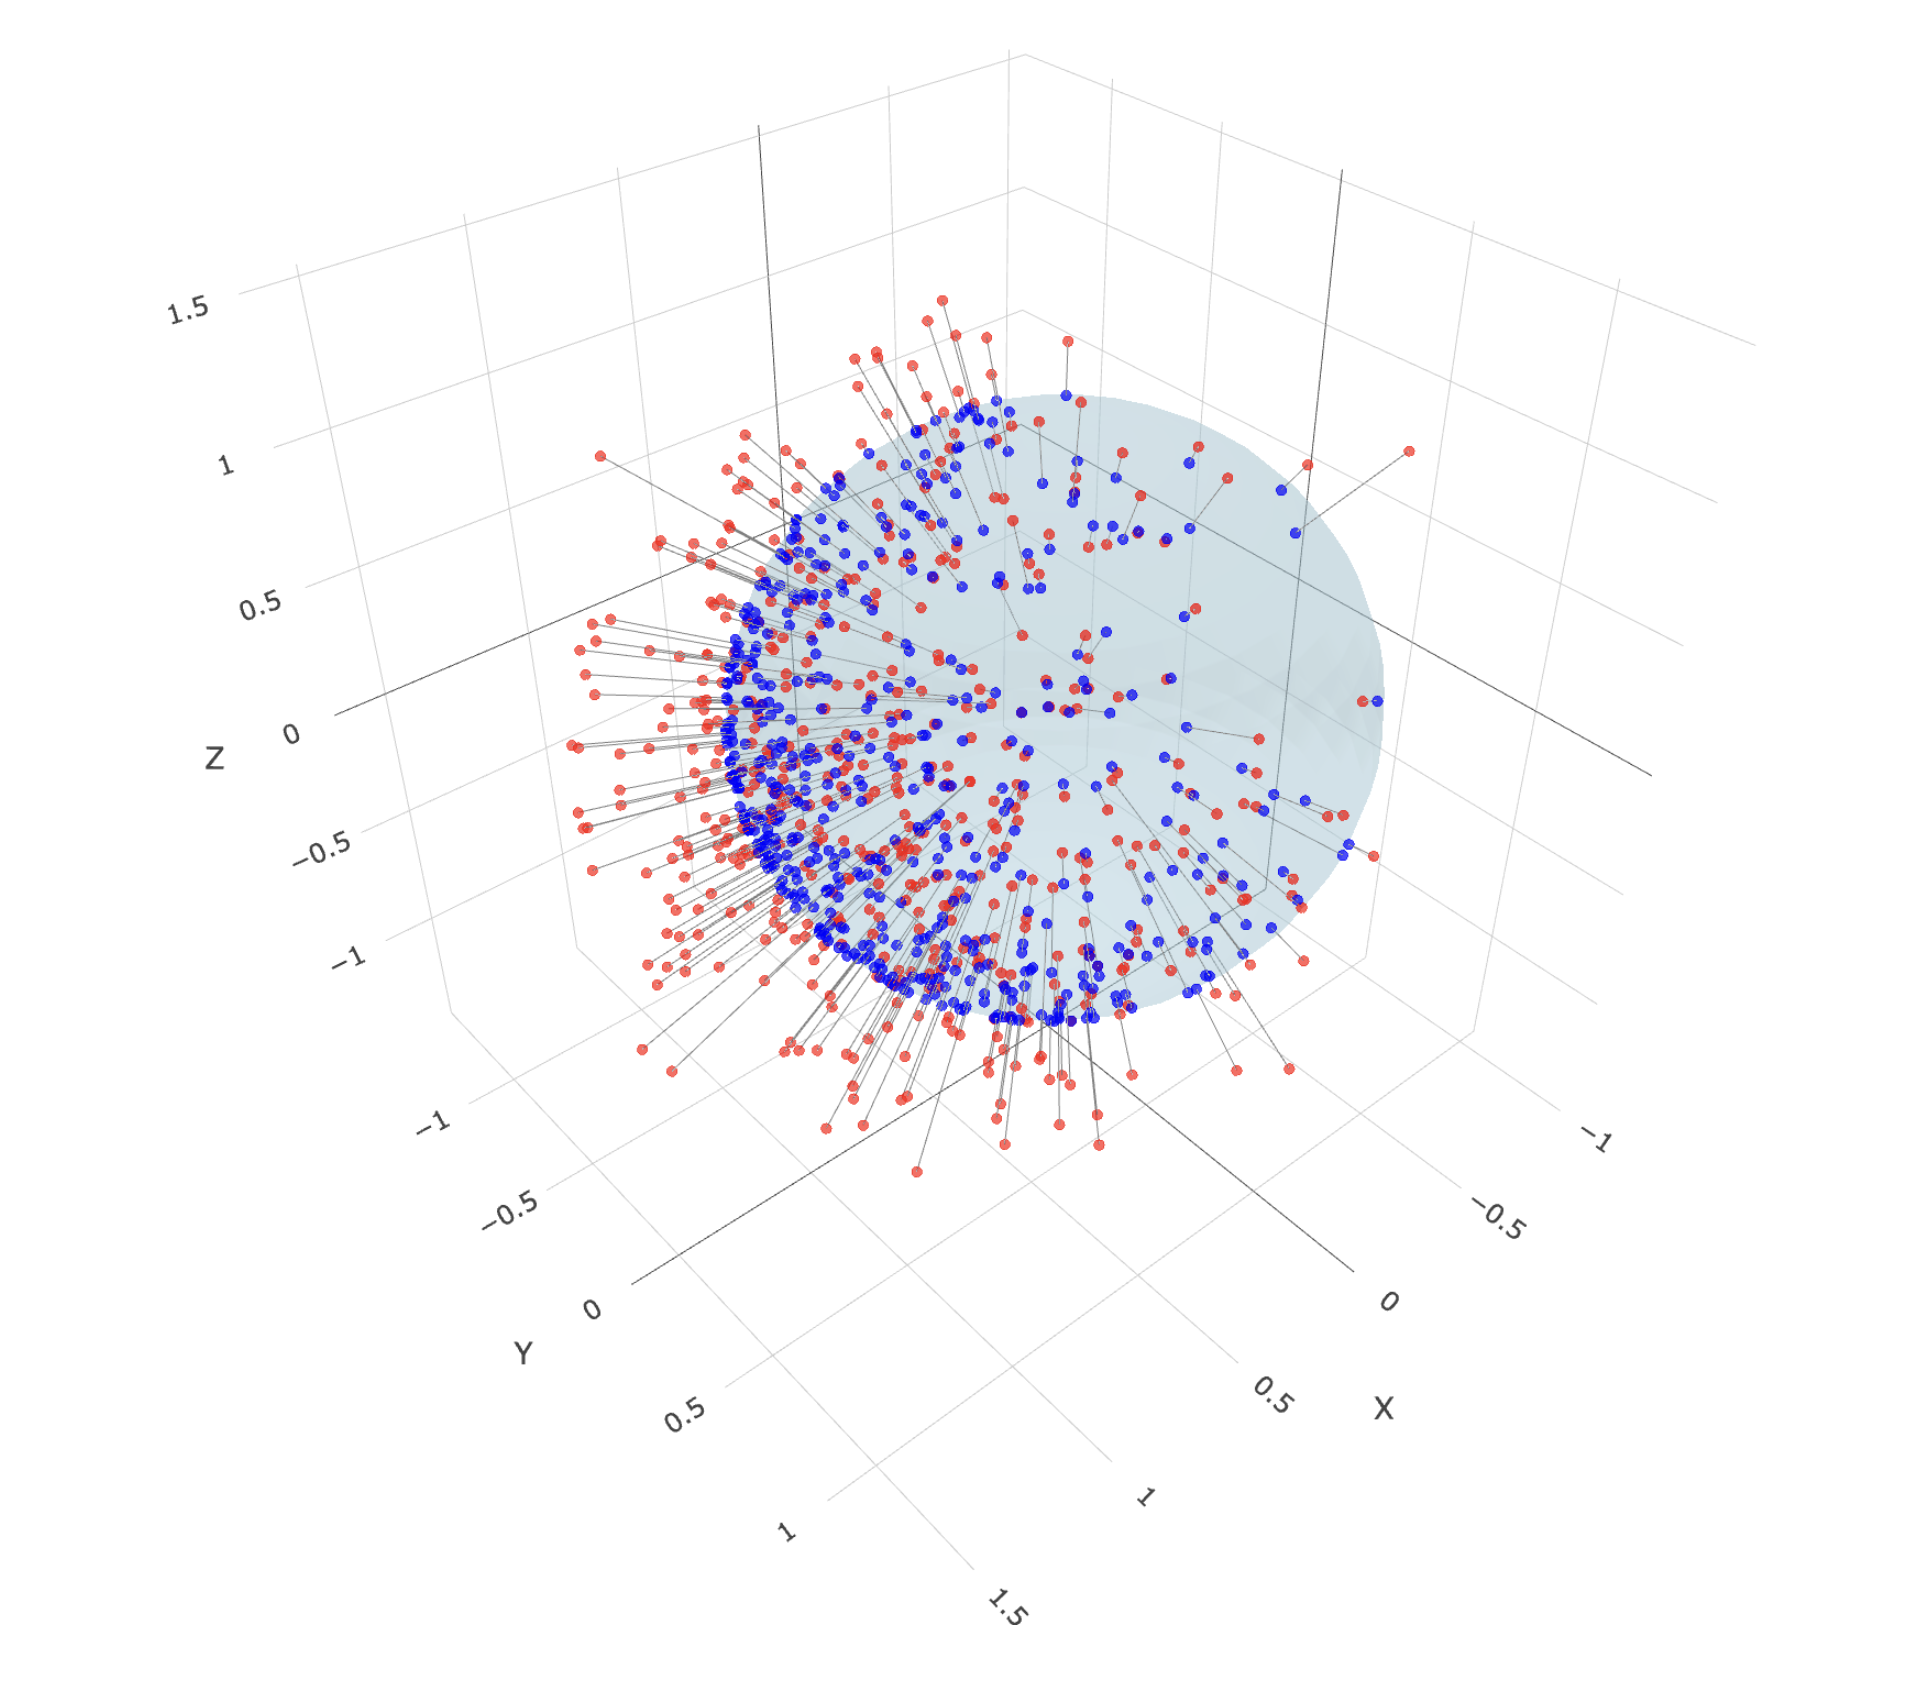
\includegraphics[width=0.75\textwidth]{../fig/data-with-noise.png}
  \end{center}
  \caption{Noisy data projected on $\mathcal{M}_3$; the unit sphere in $\mathbb{R}^3$}\label{fig:data-with-noise}
\end{figure}


\section{Directional Priors}\label{sc:directional-priors}

In contrast to the radii, the $\{D-1\}$-dimensional vector of angles, $\boldsymbol{\theta_i} := [\theta_{i, 1}, \cdots, \theta_{i, D-1}]^T$ is random. In simple terms, $\{r_i, \boldsymbol{\theta}_i\}$ is what parameterizes the realized sample $\boldsymbol{X_i} = x_i$ in space. If we draw multiple samples, the random sampling variation in $\mathbf{\theta}_i$ is what captures the randomness. In biomedical applications, such as cancer medicine, we may have reliable prior information (i.e. from previous trials or expert knowledge) on directional trends of malignant growths. Within a Bayesian framework, using our data to update these prior directional information offers a principled, probabilistic solution to complex inference problems in settings where directionality is a key piece of information.   

Before we formulate our approach formally, we briefly introduce directional statistics. When we reparameterized our data from Cartesian coordinates into polar coordinates, we did not address the underlying probabilistic transformations. For example, when encoding uncertainty in a spherical setting, it may be naive to parameterize a normal density with support on $\mathbb{R}^1$ since angles are defined in the interval $[0, 2\pi]$. Directional statistics offer well-defined spherical reparameterizations of distributions, such as the normal. Instead of defining a mean vector in $\mathbb{R}^1$, we can define a mean directional vector contained in $[0, 2\pi]$. To account for the infinite support, the wrapped normal is defined on a support of $k\text{mod}(2\pi)$. Henceforth, unless stated otherwise, we will deal with the spherical parameterizations of densities to account for the spherical parameterization of our problem. 

\subsection{Motivating Example: 3D Sphere}

We begin our discussion with an example of a 3D sphere. As discussed, this means that we have some simulated noisy data $\{x_i\}_{i=1}^n$ in 3D space. The noisy data is projected on the manifold of choice, i.e. the unit sphere. This yields the data $\{f(x_i)\}_{i=1}^n$. These data are parameterized in a polar coordinate system with $\{r_i, \mathbf{\theta}_i\}$, where the (non-random) radius $\vec{r_i}$ is the vector from the origin to $f(x_i)$. Since we are in 3D space, we have two angles. One angle, $\{\mathbf{\theta}\}_{i=1}^n$, which parameterizes the angle from the origin on the XY-plane. The angle $\{\mathbf{\phi}\}_{i=1}^n$ is the angle between the XY-plane and the point $f(x_i)$. 

\begin{figure}[h!]
  \begin{center}
    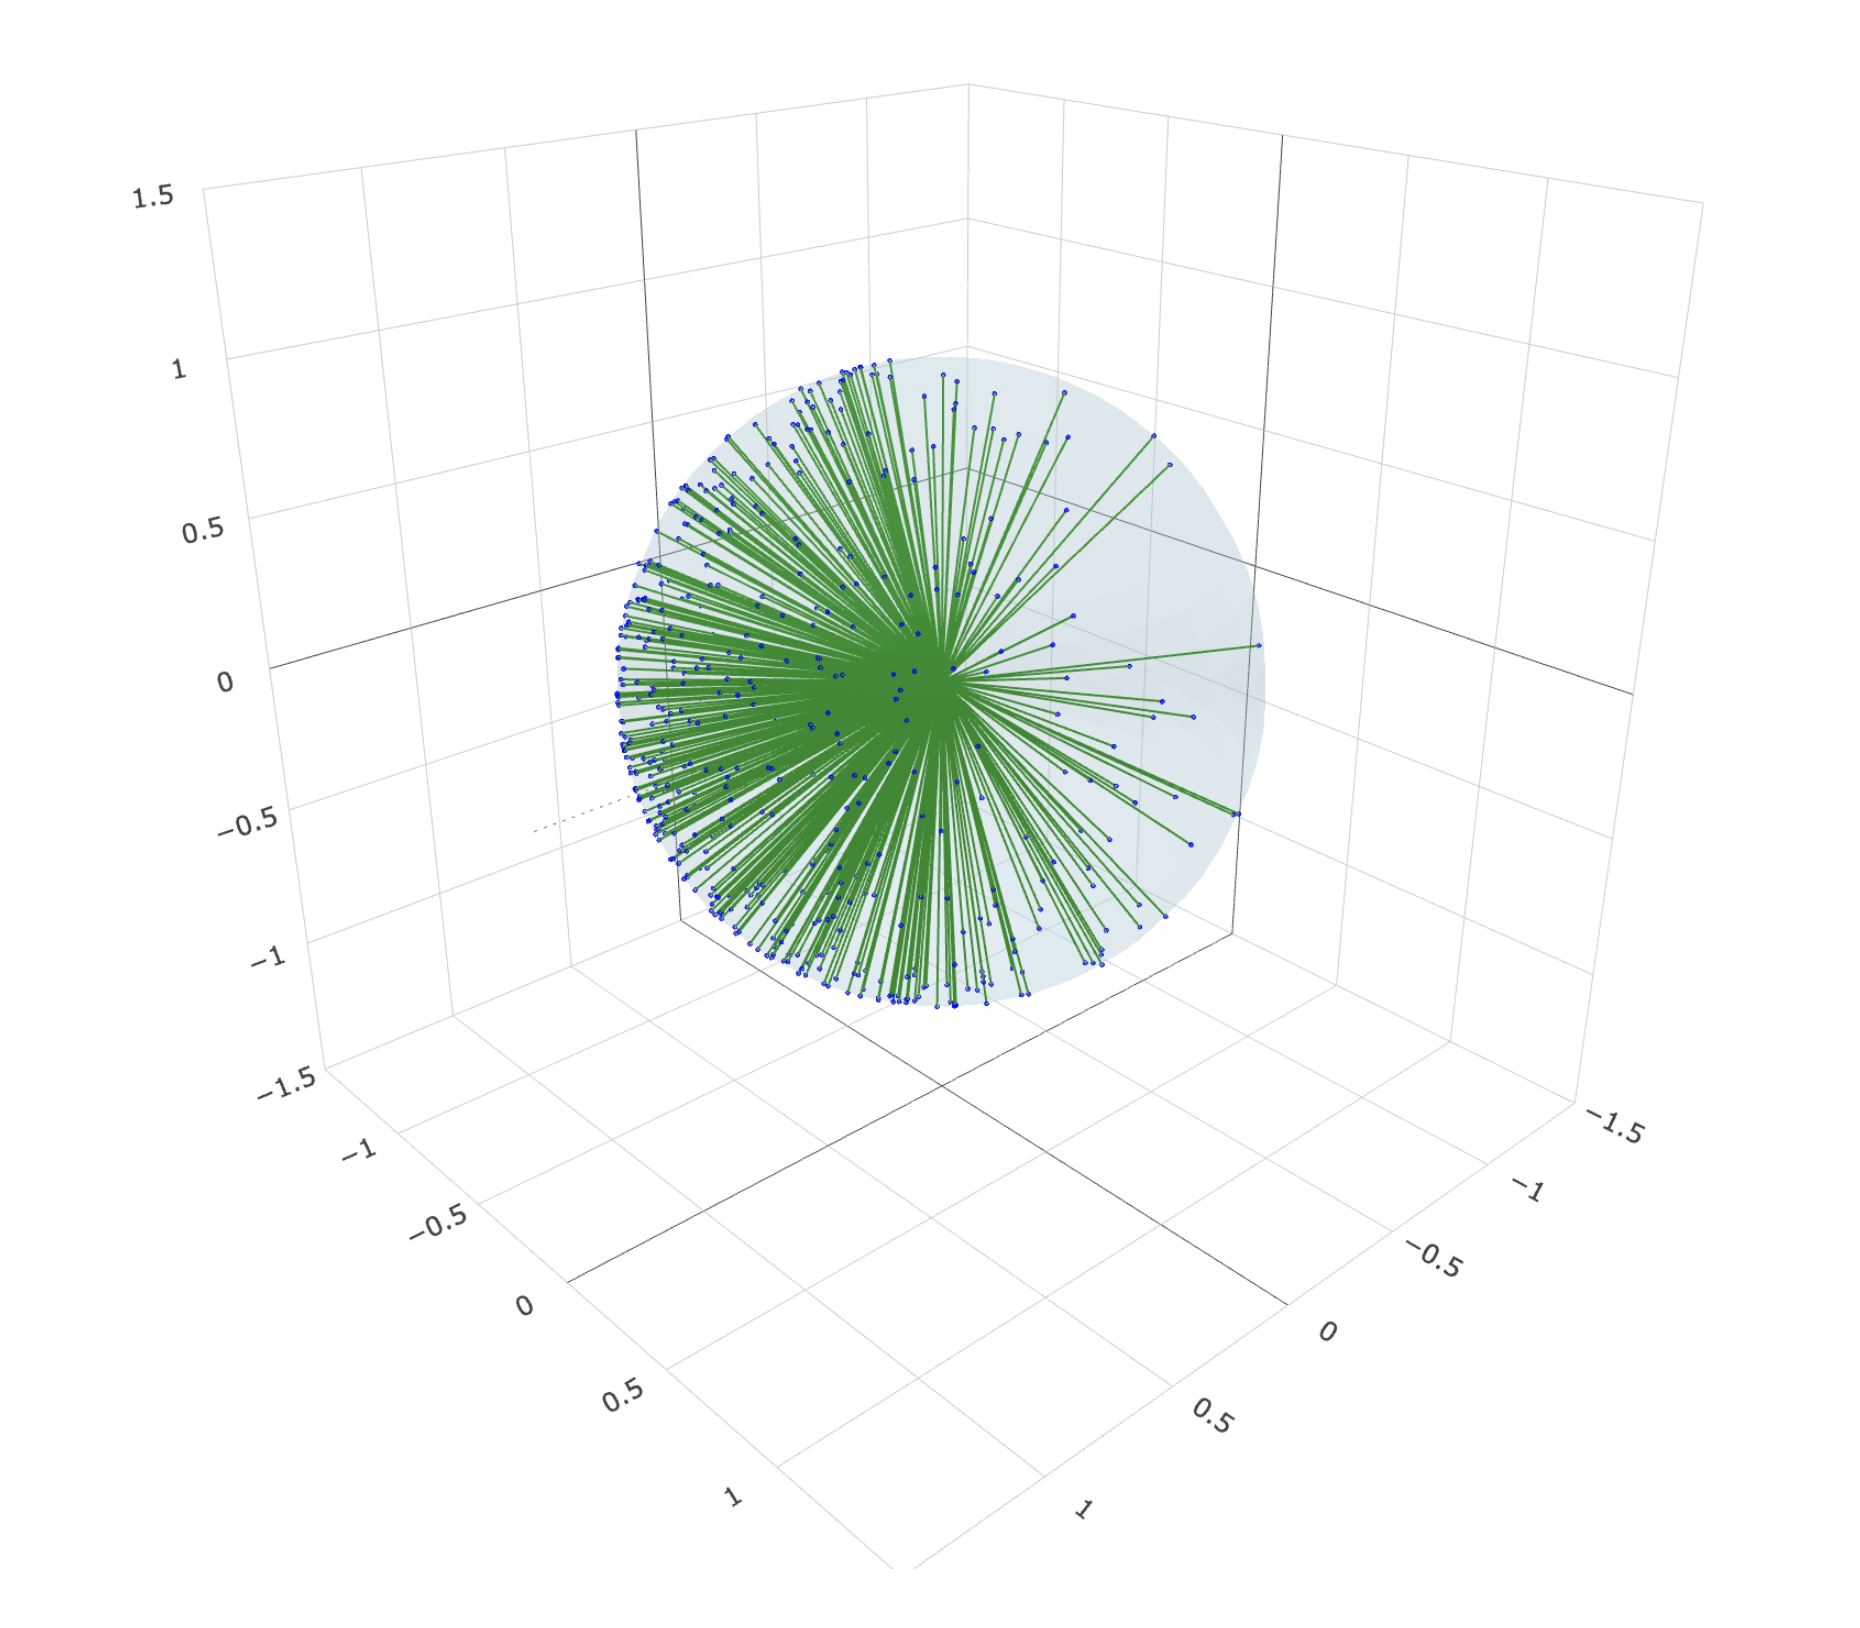
\includegraphics[width=0.75\textwidth]{../fig/projections-from-origin.png}
  \end{center}
  \caption{Polar parameterization with $\{r_i, \theta_i, \phi_i\}$ of projected data}\label{fig:projections-from-origin}
\end{figure}

\subsection{Formulating Directional Priors}\label{sc:dir-priors}

Formulating a directional prior requires careful consideration of reference points. All angles must be measured from the same reference point—for simplicity, we choose the origin. A directional prior with mean direction $\mu \in [0, \pi]$ allows us to incorporate information about where projected points should concentrate on the manifold. We only posit a prior on the random set $\{\theta_i\}_{i=1}^n$, expressing prior distributional beliefs on point concentrations in the XY-plane. For this example, we consider angles $\{\phi_i\}_{i=1}^n$ fixed, making our example univariate. Extension to the multivariate case is straightforward using multivariate analogs of our likelihood and prior distributions.

Our posterior distribution on the random vector $\theta$ can be expressed as:

$$
\begin{aligned}
  f_{\theta | \mu} (\theta | \mu) 
  &\propto \left\{ \prod_{i=1}^n f_{\theta_i | \mu}(\theta_i | \mu) \right\} \cdot f_{\mu}(\mu) \\ 
  &\propto \mathcal{L}(\theta | \mu) \cdot f_{\mu}(\mu) 
\end{aligned}
$$

where $\mu$ is our mean vector with prior $\mu \sim f_{\mu}(\mu)$. For our likelihood, we initially consider the wrapped normal distribution with density:

$$
f(\theta|\mu,\sigma^2) = 
\frac{1}{2\pi\sigma^2} \sum_{k=-\infty}^{\infty} \exp\left(-\frac{(\theta-\mu+2\pi k)^2}{2\sigma^2}\right)
$$

However, this infinite series presents computational challenges. Instead, we use the von Mises distribution, which provides a more tractable circular analog to the normal distribution:

$$
f(\theta|\mu,\kappa) = \frac{e^{\kappa \cos(\theta-\mu)}}{2\pi I_0(\kappa)}
$$

where $\theta$ is the angle, $\mu$ is the mean direction, $\kappa \geq 0$ is the concentration parameter (analogous to precision, or inverse variance), and $I_0(\kappa)$ is the modified Bessel function of first kind of order 0. As $\kappa$ increases, the distribution concentrates more tightly around $\mu$. When $\kappa = 0$, the distribution becomes uniform on the circle. The von Mises distribution scales naturally for hyperspheres in $\mathbb{R}^p$, making it ideal for spherical settings in manifold learning applications.

\subsection{Variance Encodes Curvature}\label{sc:curvature}

For our concentration parameter $\kappa$, naive selection (e.g., a constant) would be possible but would negate the benefits of manifold learning as a topology-preserving dimensionality reduction technique. Instead, we propose a principled approach that encodes local topological structure into the variance parameter. Intuitively, in regions with little topological variation, we might update our projection more liberally. Conversely, if a small change in projection angle moves our data point into a topologically distinct region, we would be more conservative with updates.

In spherically parameterized manifolds, the inverse absolute Gaussian curvature provides a natural variance encoding. This approach has an elegant connection to the score test in likelihood-based inference, which uses the slope at restricted MLE estimates as a similarity measure. Thus, our solution has both topological intuition and established statistical parallels in traditional inference methods.

The Gaussian curvature of a surface can be defined as the product of the principal curvatures:

$$K = k_1 \cdot k_2$$

where $k_1$ and $k_2$ are the principal curvatures at a point on the surface. For a sphere of radius $R$, due to perfect symmetry, both principal curvatures equal $\frac{1}{R}$, giving a Gaussian curvature of $K = \frac{1}{R^2}$. For a unit sphere, the Gaussian curvature is $K = 1$, an intrinsic property related to the total curvature integrated over the entire sphere equaling $4\pi$ by the Gauss-Bonnet theorem.

\begin{figure}[h!]
  \begin{center}
    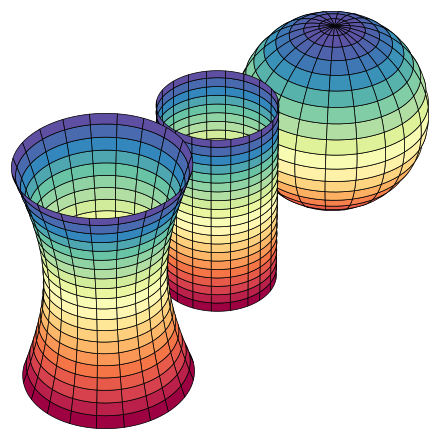
\includegraphics[width=0.5\textwidth]{../fig/gaussian-curvature.png}
  \end{center}
  \caption{From left to right: a surface of negative Gaussian curvature (hyperboloid), a surface of zero Gaussian curvature (cylinder), and a surface of positive Gaussian curvature (sphere).}\label{fig:gaussian-curvature}
\end{figure}

This curvature-based approach provides a meaningful way to weight observations based on their location in the manifold's topological structure. Areas with high curvature (significant bending of the manifold) will contribute less to updating our beliefs than areas with lower curvature (flatter regions), which aligns with our geometric intuition about confidence in projections.

\subsection{Conjugacy Results}\label{sc:conjugacy}

A key advantage of the von Mises distribution is conjugacy, which allows for straightforward Bayesian updates of our directional priors. Following the work of \citet{mardia1976}, a von Mises prior with mean direction $\mu$ and concentration parameter $\kappa$ is conjugate to the likelihood. After observing angles $\theta_1,\ldots,\theta_n$, the posterior distribution takes the form:

$$
f(\mu_i, \mu^* | \{\theta_i\}_{i=1}^n) \propto \exp(\kappa \cdot \sum_{i=1}^n \cos(\theta_i - \mu_i) +\kappa^* \cdot \sum_{i=1}^n \cos(\mu_i - \mu^*))
$$

where angles $\{\theta_i\}_{i=1}^n \sim \mathcal{VM}(\mu_i, \kappa)$ and the prior is $\mu_i \sim \mathcal{VM}(\mu^*, \kappa^*)$. In our case, the data were generated with $\mu_i = \mu = \text{circular}(0)$.

The posterior form reveals a shrinkage estimator structure. The component involving observed angles $\{\theta_i\}_{i=1}^n$ is weighted by $\kappa$, which in our framework represents the curvature at the projected point. The difference between the data mean and prior mean is weighted by the prior concentration parameter $\kappa^*$. This structure extends shrinkage estimation to our topological interpretation: when the data concentration parameter $\kappa$ is low, more weight is attributed to our prior information.

For our 3D spherical example, given a prior $\boldsymbol{\theta} \sim \mathcal{VM}(\theta_0, \tau_0 = \frac{1}{\kappa_0})$, the posterior mean is:

$$
\underbrace{\frac{\tau_0}{\tau_0 + \hat{\tau}} \cdot \theta_0}_{\text{Weighted Prior Vector}} + \underbrace{\frac{\hat{\tau}}{\tau_0 + \hat{\tau}} \cdot \bar{\theta}}_{\text{Weighted Data Vector}}
$$

with posterior variance $(\tau_0 + \hat{\tau})^{-1}$, where $\bar{\theta} := \frac{1}{n}\sum_{i=1}^n \theta_i$ and $\hat{\tau} = \frac{1}{\hat{\kappa}}$ with $\hat{\kappa}$ being the observed Gaussian curvature at the manifold point. The shrinkage toward the prior mean is immediately evident in this expression.

\begin{figure}[h!]
  \begin{center}
    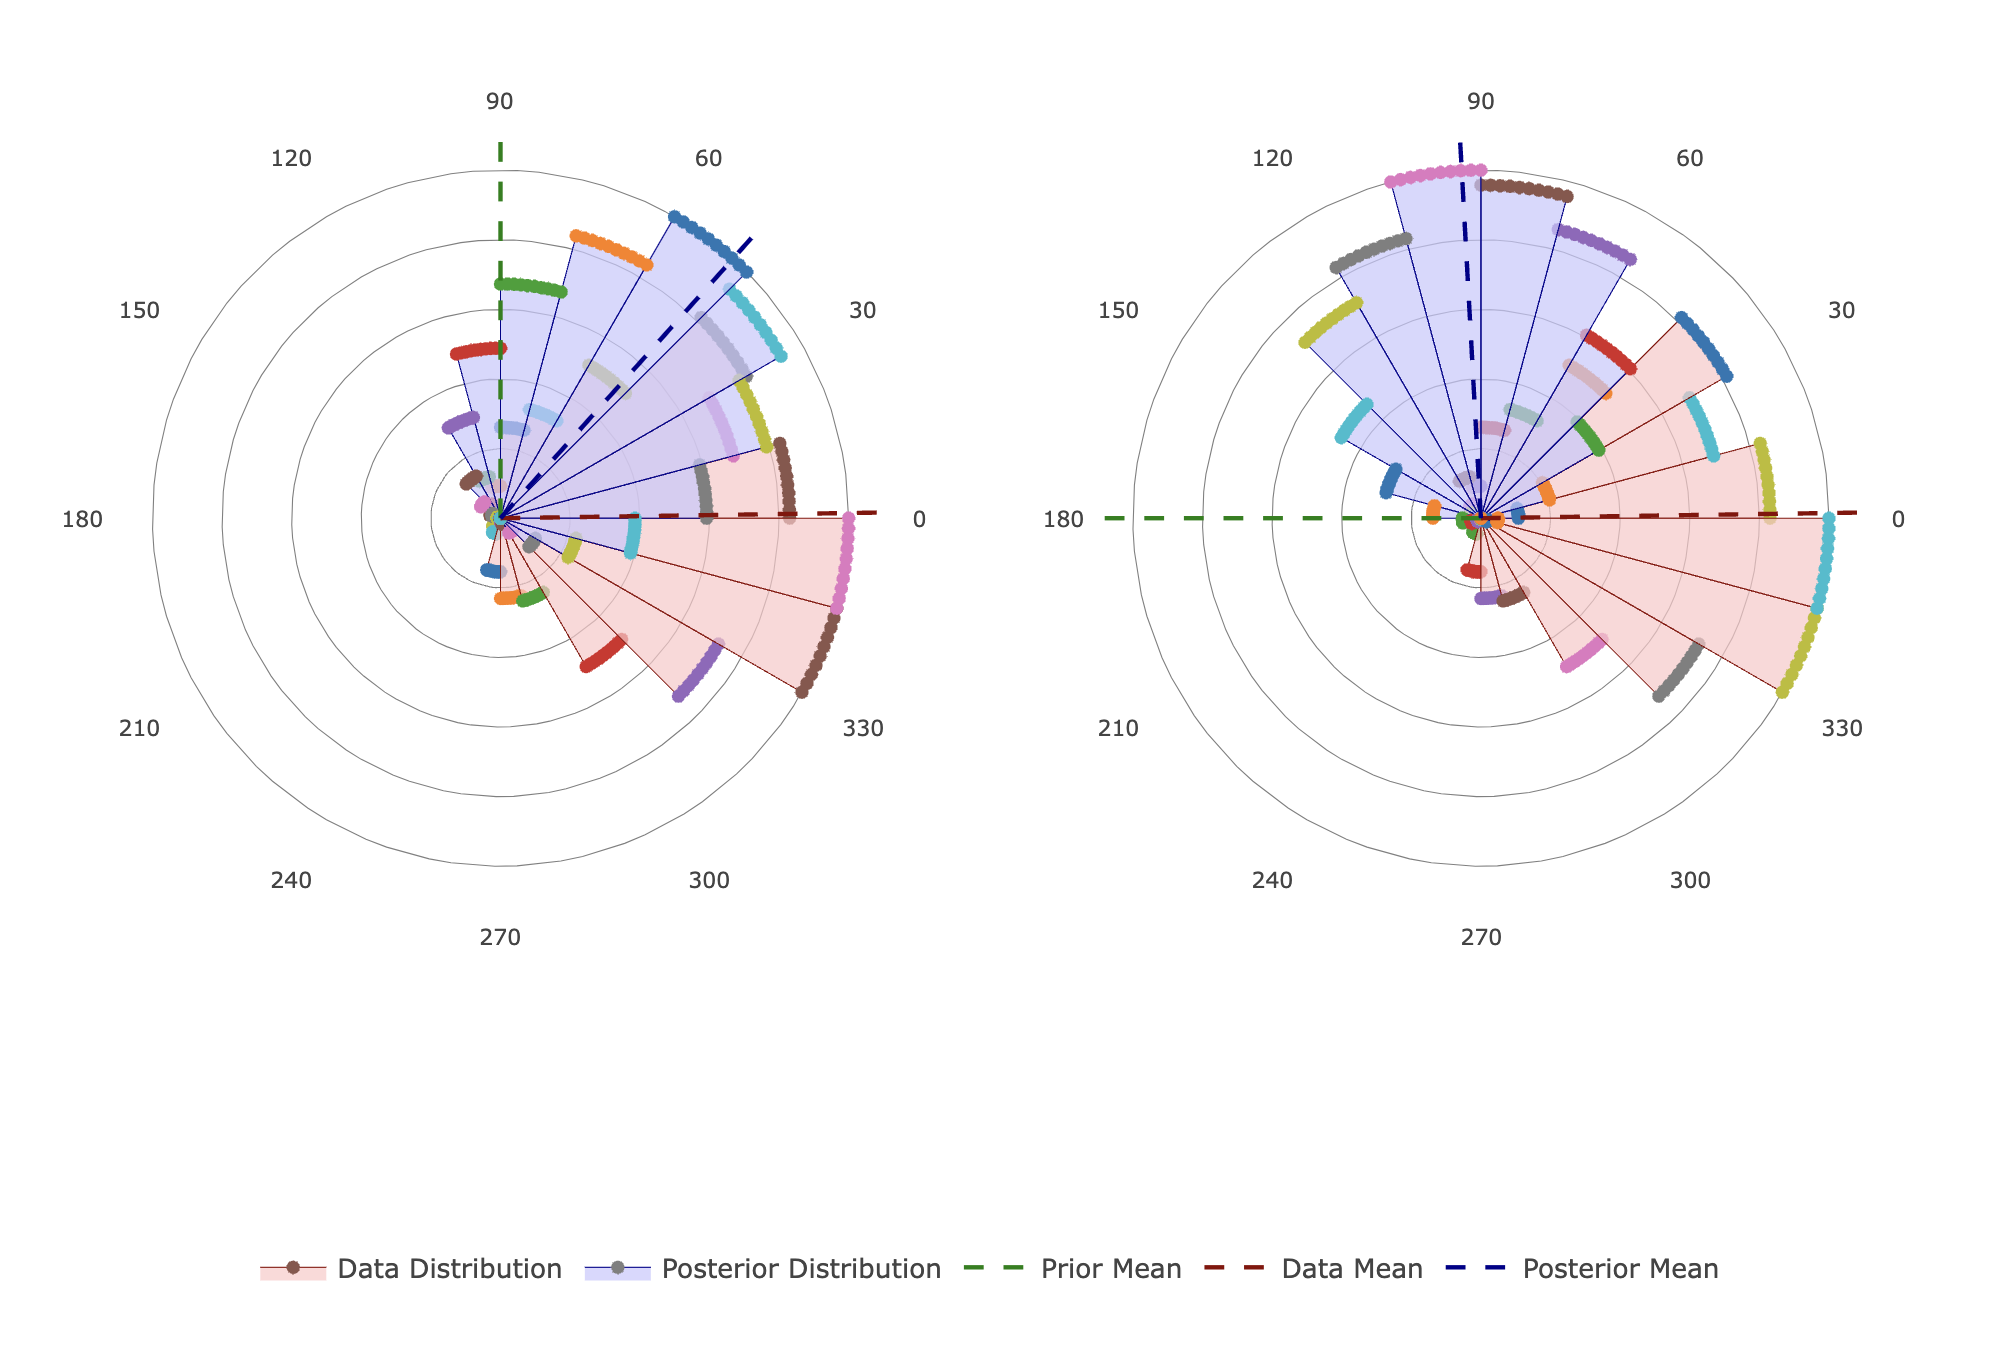
\includegraphics[width=1\textwidth]{../fig/posterior-roseplot.png}
  \end{center}
  \caption{Posterior distribution under prior $\theta_0$: Left $\theta_0 = \pi/2$; Right: $\theta_0 = \pi$}\label{fig:posteriors}
\end{figure}

Figure \ref{fig:posteriors} demonstrates that the posterior mean effectively balances the prior and data means. This occurs because our manifold is a sphere with equivalent curvature at every point. For manifolds with heterogeneous curvature, we would observe less reprojection with respect to the prior mean in regions where curvature is more extreme, thus preserving the topological characteristics of the data.

The conjugacy relationship for von Mises distributions has an elegant geometric interpretation. For a von Mises likelihood $f(x|\mu) \propto \exp(\kappa \cos(x-\mu))$ and a von Mises prior on the mean direction $\pi(\mu) \propto \exp(\kappa_0 \cos(\mu-\mu_0))$, the posterior distribution is also von Mises: $\pi(\mu|x) \propto \exp(\kappa_n \cos(\mu-\mu_n))$. The posterior parameters can be expressed in terms of resultant vectors:

$$\kappa_n\cos(\mu_n) = \kappa_0\cos(\mu_0) + \kappa\cos(x)$$
$$\kappa_n\sin(\mu_n) = \kappa_0\sin(\mu_0) + \kappa\sin(x)$$

These equations can be rewritten in vector form as:

$$\kappa_n = \sqrt{(\kappa_0\cos(\mu_0) + \kappa\cos(x))^2 + (\kappa_0\sin(\mu_0) + \kappa\sin(x))^2}$$

and 

$$\mu_n = \text{atan2}(\kappa_0\sin(\mu_0) + \kappa\sin(x), \kappa_0\cos(\mu_0) + \kappa\cos(x))$$

This representation yields a powerful geometric interpretation: the posterior mean direction and concentration are determined by the vector sum of the prior and likelihood information vectors in $\mathbb{R}^2$. Each vector has direction given by unit vectors pointing at angles $\mu_0$ and $x$ respectively, with magnitude determined by concentration parameters $\kappa_0$ and $\kappa$. The resultant vector's length determines the posterior concentration parameter $\kappa_n$, while its direction determines the posterior mean direction $\mu_n$. 

This insight demonstrates that when prior and likelihood point in similar directions, the posterior becomes more concentrated (higher $\kappa_n$), reflecting increased certainty. Conversely, conflicting directions lead to a less concentrated posterior (lower $\kappa_n$), reflecting uncertainty.

The posterior mean naturally represents a weighted compromise between prior and data, with weights proportional to their respective concentration parameters. For multiple observations, the vectors from each observation simply add to the prior vector, providing an efficient sequential updating mechanism. This vector-based interpretation elegantly connects Bayesian inference on the circle with vector addition in the plane, making it particularly suitable for our manifold learning framework where directional data naturally arises from projections onto curved surfaces.

\section{A Causal Extension -- Toward a Manifold RD Estimator}\label{sc:causal}

\textcolor{red}{Make it crystal clear that the posterior variance is the Bayesian thing here!!}

An interesting application of directional priors is a causal setting where we seek to estimate treatment effects after some treatment has been administered. A popular class of estimators for comparing changes in outcomes of interest close to a treatment cut-off are regression discontinuity (RD) estimators. RD estimators exploit the the balance between units close to the treatment cut-off, assuming that treatment does not depend on any unit characteristics. Recovering causal effects in RD estimators hinges on the assumption that in terms of unit characteristics, treatment assignment is quasi-random very close to the cut-off. Popular examples in literature include measuring the effect of advanced coursework on students above some cutoff, comparing their outcomes to students just below said cutoff. 

In the principal manifold learning setup, directional priors offer a promising Bayesian approach to causal inference. For simplicity, assume that treatment is administered at time point $t^*$. Then, all units in $(-\infty, t^*)$ are pre-treatment units, and all units in $[t^*, \infty)$ are post-treatment units. In a canonical RD setting, under a set of identification assumptions, we can recover an average treatment by considering values of $Y_i$ immediately to the right (say $Y_{it} |_{t^* + \delta}$) and left ($Y_{it} |_{t^* - \delta}$) of the cutoff. This yields the causal estimate  

$$
\hat{\tau}= \bar{Y}|_{t = t^* + \delta} - \bar{Y}|_{t = t^* - \delta} 
$$

The above estimator is commonly measured in the Local Linear Regression (LLR) framework, i.e. measure the ATE as the difference in post- and pre-treatment means, given that they are sufficiently close to the treatment cutoff $t^*$. \citet{Branson2019} considers a Bayesian RD setting where a Gaussian process prior is placed on the pre- and post-treatment mean response functions. We believe this work, although not directly related to the use of topological information in causal inference, encapsulates the desire for more flexible, data-driven, and principled causal inference through Bayesian paradigms.   

\subsection{Intuition}

In a principal manifolds framework, we can also exploit this notion of quasi-randomness to recover causal effects. Specifically, we propose the estimation of causal treatment effects using the posterior density of projection angles with empirical prior variances encoding the local topological structure of pre-treatment manifolds. For this procedure, suppose we use the set of pre-treatment units $\{Y_{it}\}_{i=1}^n|_{t < t^*}$ to fit the $d$-dimensional manifold $\mathcal{M}_d^{t < t^*}$. As we have shown in Section~\ref{sc:directional-priors}, a polar reparameterization allows us to recover the projection angles $\{\theta_i\}$ as well as their mean which we shall denote as $\bar{\theta}^{t < t^*}$. This mean pre-treatment projection angle $\bar{\theta}^{t < t^*}$ has a curvature which we will denote as $\kappa^{t<t^*}$. Together, the mean pre-treatment projection angle and curvature sufficiently parameterize the first two moments of the pre-treatment outcome of interest. 

After treatment happens at $t=t^*$, we can fit the post-treatment manifold $\mathcal{M}_d^{t \geq t^*}$. In the spirit of LLR-based causal estimation, we want to emphasize that $\mathcal{M}_d^{t \geq t^*}$ is *not* fit iteratively for each post-treatment unit, i.e. we do not obtain the post-treatment unit by combining the post-treatment units with pre-treatment units. Instead, our pre- and post-treatment manifolds are topological analogues to $\bar{Y}|_{t = t^* - \delta}$ and $\bar{Y}|_{t = t^* + \delta}$, respectively. That being said, it may be interesting to let the choice of manifold (e.g., the shape, highest order, etc.) from the pre-treatment case inform the post-treatment case, effectively borrowing prior topological information on a more global level. \footnote{This is a really interesting direction in the Bayesian paradigm and touches on the notion of persistent homology. Although this discussion goes beyond the scope of this paper, it highlights how nuanced various levels/ sources of topological information can be.} Now, suppose that we observe the outcomes of $m$ additional units in the immediate post-treatment period, then the data $\{Y_{it}\}_{i=n+1}^{m}|_{t \geq t^*}$ allows us to fit the manifold $\mathcal{M}_d^{t \geq t^*}$. The mean projection angle of $\mathcal{M}_d^{t \geq t^*}$, i.e. $\bar{\theta}^{t \geq t^*}$ will update from $\bar{\theta}^{t < t^*}$, and yield a new posterior estimate for the projection angle.  

\begin{figure}
  \begin{center}
\begin{tikzpicture}[scale=0.9]
    % Define colors
    \definecolor{darkgrey}{RGB}{80,80,80}
    \definecolor{darkorange}{RGB}{204,85,0}
    
    % Time axis
    \draw[->, thick] (-0.5,0) -- (10.5,0) node[right] {$t$};
   
    % Pre-treatment and post-treatment labels
    \node[align=center, text width=4cm] at (2.5,-0.5) {\text{Pre-treatment}};
    \node[align=center, text width=4cm] at (7.5,-0.5) {\text{Post-treatment}}; 
    
    % Treatment cutoff vertical line
    \draw[dashed, thick] (5,0) -- (5,7);
    \node at (5,-0.5) {$t^*$};
    
    % Pre-treatment manifold as a regular ellipse (dark grey)
    \draw[thick, darkgrey] (2.5,3) ellipse (1.5 and 2);
    \node[darkgrey] at (2.5,5.7) {$\mathcal{M}_d^{t < t^*}$};
    
    % Pre-treatment projection angle (dark grey)
    \draw[->, thick, darkgrey] (2.5,3) -- (3.5,4.4);
    \node[darkgrey] at (4.2, 4.5) {$\bar{\theta}^{t < t^*}$};
    
    % Post-treatment: ghost of pre-treatment manifold (dashed)
    \draw[thick, dashed, darkgrey] (7.5,3) ellipse (1.5 and 2);
    
    % Post-treatment manifold as a pointier ellipse, rotated 12 degrees (darkorange)
    \begin{scope}[shift={(7.5,3)}, rotate=12]
        \draw[thick, darkorange] (0,0) ellipse (1.2 and 2.2);
    \end{scope}
    \node[darkorange] at (7.5,5.7) {$\mathcal{M}_d^{t \geq t^*}$};
    
    % Two projection angles in post-treatment period
    \draw[->, thick, darkorange] (7.5,3) -- (7.8,4.85);  % Updated angle (darkorange)
    \node[darkorange] at (8.5, 5.2) {$\bar{\theta}^{t \geq t^*}$};
    \draw[->, thick, darkgrey] (7.5,3) -- (8.6,4.4);  % Original angle direction (dashed, dark grey)
     \node[darkgrey] at (9.4, 4.5) {$\bar{\theta}^{t < t^*}$};
    
    % Data points on pre-treatment manifold (dark grey)
    \foreach \x/\y in {1.5/3.5, 2/2, 3/2, 3.5/3.5, 2.5/4.5, 2.5/1.5} {
        \fill[darkgrey] (\x,\y) circle (2pt);
    }

    % Data points on post-treatment manifold (dark grey)
    \foreach \x/\y in {6.8/3.8, 7/2, 8/2.2, 8.3/3.7, 7.5/4.8, 7.3/1.3, 7/5} {
        \fill[darkorange] (\x,\y) circle (2pt);
    }
    
    % Legend
    \begin{scope}[shift={(0,-1.5)}]
        % Rectangle around the legend - made even wider
        \draw[black] (0,0) rectangle (11,-1.5);
        
        % Legend title
        %\node[align=center] at (5.5,-.3) {\textbf{Legend}};
        
        % Pre-treatment elements (darkgrey)
        \draw[thick, darkgrey] (1.5,-0.7) -- (2.5,-0.7);
        \node[darkgrey, align=left, text width=7.5cm] at (6.8,-0.7) {Pre-treatment manifold and projection};
        
        % Post-treatment elements (darkorange)
        \draw[thick, darkorange] (1.5,-1.2) -- (2.5,-1.2);
        \node[darkorange, align=left, text width=7.5cm] at (6.8,-1.2) {Post-treatment manifold and projection};
    \end{scope} 
  \end{tikzpicture}
  \end{center}
  \caption{The Manifold RD Estimator}\label{fig:manifold-rd}
\end{figure}

\subsection{The Estimator}

Combining our insights from RD estimators with the conjugacy results of Section~\ref{sc:conjugacy}, we propose a Bayesian manifold RD estimator in its simplest form. After having the pre- and post-treatment manifold, consider subtracting the pre-treatment distribution of angles from the post-treatment distribution. This yields a RD estimator of the form: 

$$
f_{\tau | \theta} = 
\mathcal{VM}
\left(
  \bar{\theta}^{t \geq t^*} - \bar{\theta}^{t < t^*}, \sigma^2 
\right)
$$ 

where 

\[
  \sigma^2 = \sqrt{\left[\kappa^{t < t^*}\cos(\bar{\theta}^{t < t^*}) + \textcolor{darkorange}{\kappa^{t \geq t^*}\cos(\bar{\theta}^{t \geq t^*})}\right]^2 
  + 
\left[\kappa^{t < t^*}\sin(\bar{\theta}^{t < t^*}) + \textcolor{darkorange}{\kappa^{t \geq t^*}\sin(\bar{\theta}^{t \geq t^*})}\right]^2}
\]

by the conjugacy results of Section~\ref{sc:conjugacy}. 

Here, we estimate the Average Treatment Effect (ATE) as the difference between the mean projection angles of the post- and pre-treatment manifold, respectively. As illustrated in Figure~\ref{fig:manifold-rd}, this difference captures the directional shift in data geometry following treatment intervention. The posterior variance, expressed as the Euclidean norm of the difference between weighted directional vectors, quantifies our uncertainty about this effect. Intuitively, a larger norm indicates greater topological dissimilarity between pre- and post-treatment manifolds, suggesting a more substantial causal impact.

To illustrate this, let us recycle the toy example from Section~\ref{sc:conjugacy}. Suppose we have a post-treatment mean projection angle, $\bar{\theta}^{t \geq t^*} = \pi$ and a pre-treatment mean projection angle, $\bar{\theta}^{t < t^*} = \pi/2$. We consider both of these manifolds to be circles, but the post-treatment manifold has radius $2$. Thus, the manifold we have fit grows from a unit circle (radius = $1$) to a post-treatment circle with radius $2$. This means that while the pre-treatment Gaussian curvature stays 1, i.e. $\kappa^{t < t^*} = 1$, our post-treatment curvature is now $\kappa^{t \geq t^*} = \frac{1}{R^2} = \frac{1}{4}$. We simulate 500 draws and observe the following results: 

\begin{figure}[h!]
  \begin{center}
    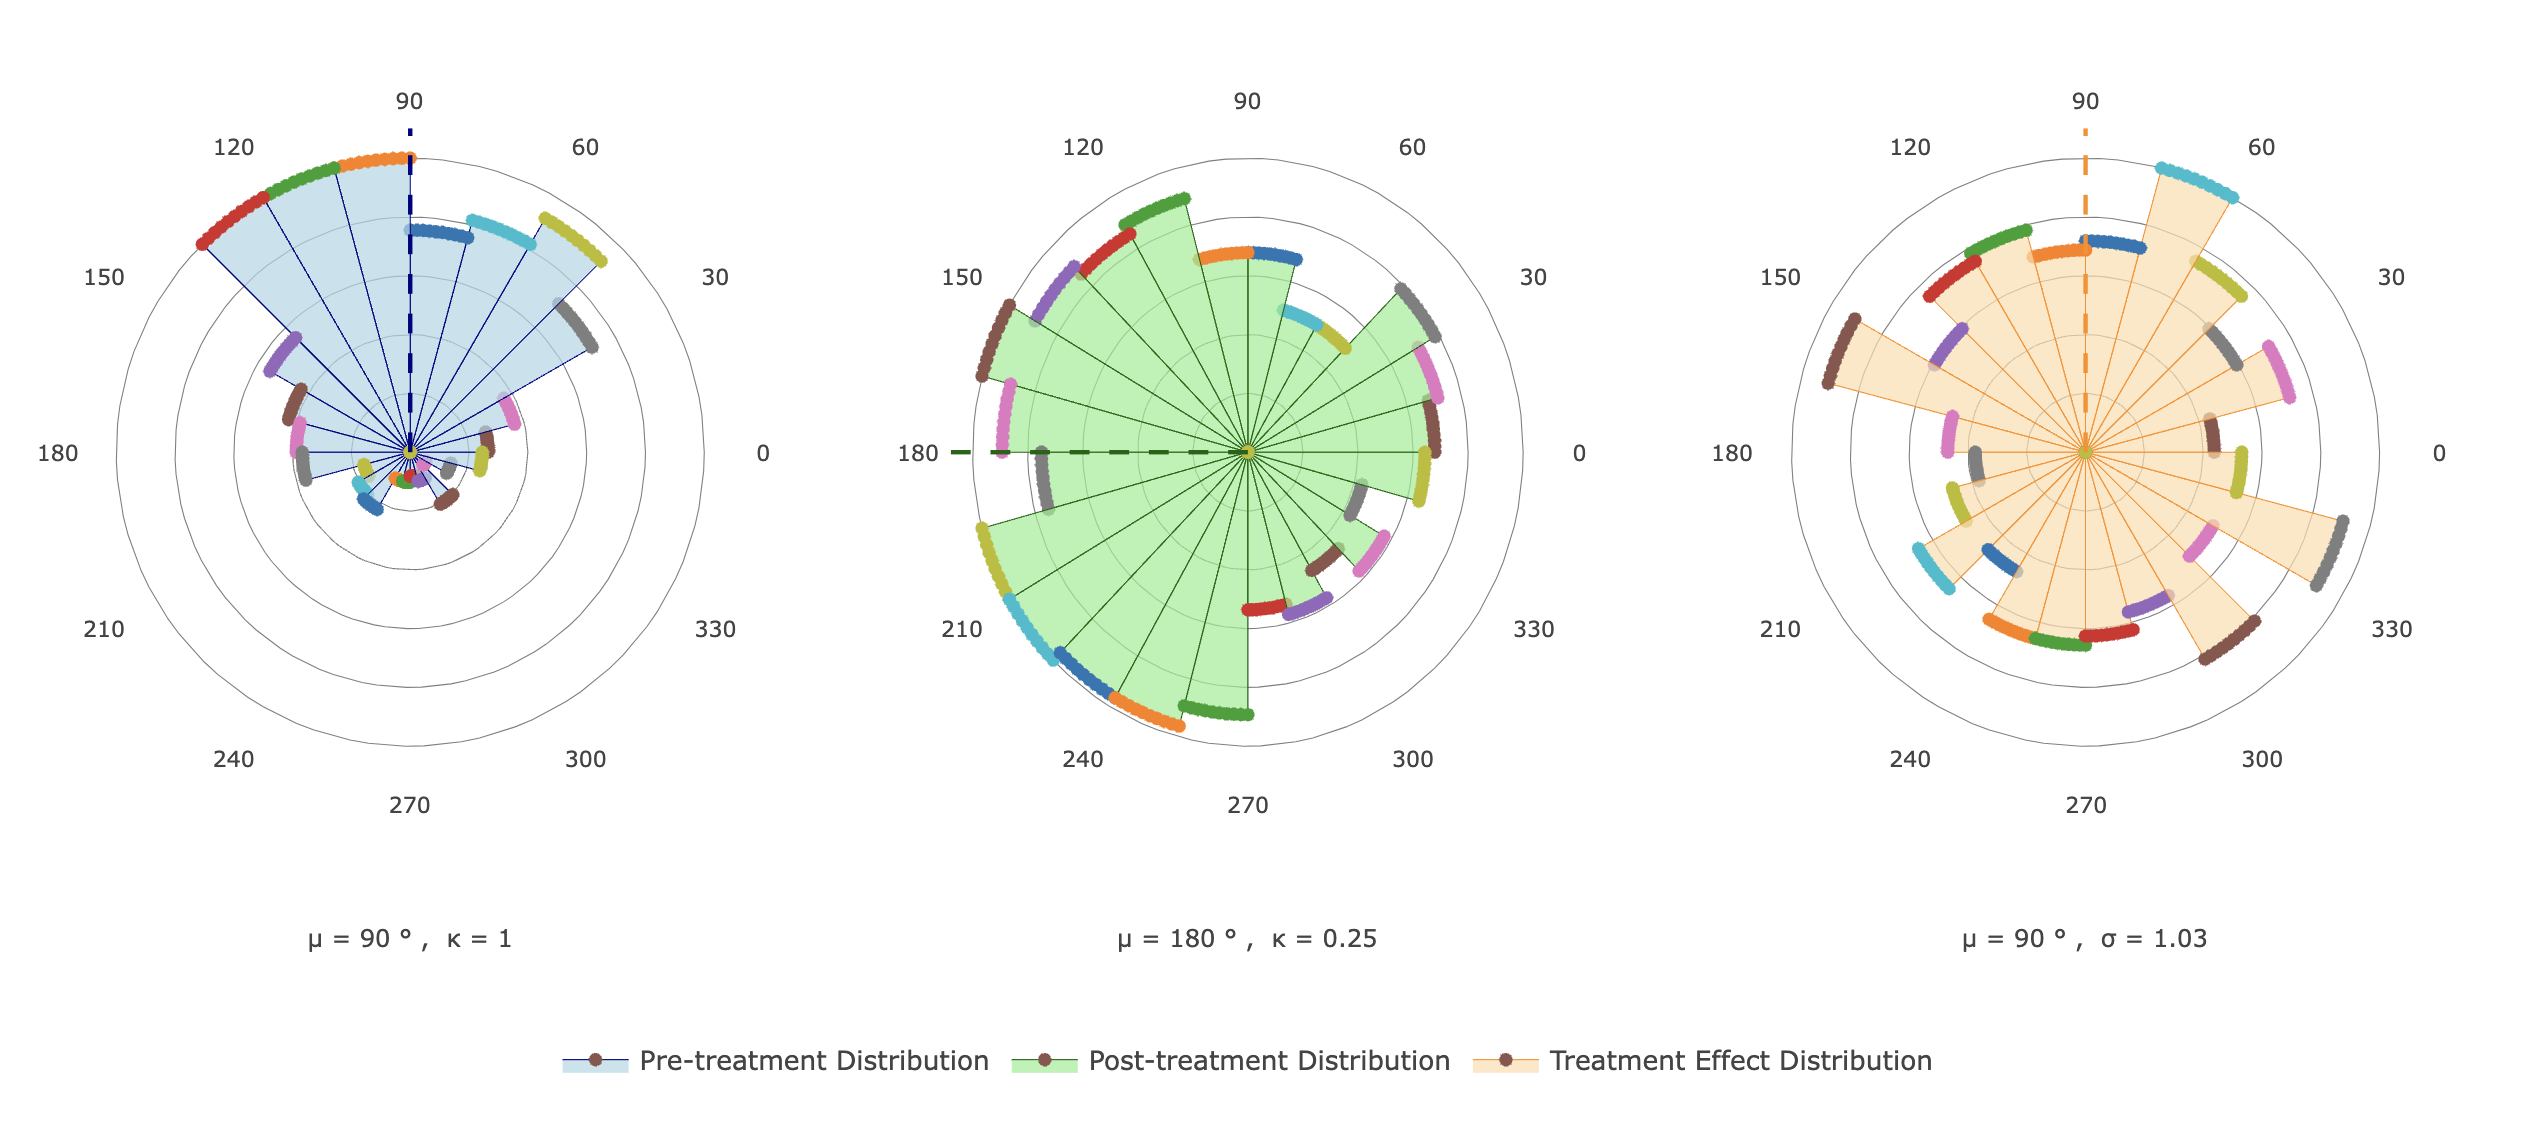
\includegraphics[width=1\textwidth]{../fig/rd-sim.png}
  \end{center}
  \caption{Simulation of Treatment Effect $\hat{\tau}$}\label{fig:rd-sim}
\end{figure}


We can see that the resulting treatment effect estimate $\hat{\tau}$ is indeed very close to $\frac{\pi}{2}$. The variance term is slightly above 1, i.e. greater than the individual parts.  

When compared to well-established LLR methods, the mean projection angles are simply a spherical reparameterization of the outcome variable of interest. This formulation naturally preserves identification assumptions required for causal interpretation while accommodating the topological abstractions within the principal manifold framework. The magnitude of the posterior variance directly reflects how drastically treatment has altered the local geometry of our outcome space, e.g., if we have a large difference, we want to encode that topological uncertainty into our ATE. 

An important point of emphasis is what this procedure is not. Namely, we are not simply updating our fitted manifold with the new data, and letting the posterior angle update iteratively with each new post-treatment observation. Rather, we are using the pre-treatment manifold to borrow topological information for our post-treatment mean vector. In that sense, after having fit $\mathcal{M}_d^{t \geq t^*}$ to the post-treatment data only, we assign the prior mean (i.e. $\bar{\theta}^{t<t^*}$) a weight of zero, only using the post-treatment observations.

We round out this section with an appealing information-theoretic point of view. This manifold RD estimate is fundamentally analogous to the existing methods. The main difference is that this procedure accounts for the topological information of our embedding space. Existing methods are quick to discard this information and assume it away. Principled manifold learning approaches combined with the flexible probabilistic advantages of Bayesian methods can therefore yield estimates that respect both prior and topological information, resulting in more flexible and data-driven inference.

\section{Limitations and Future Direction}

Future work could address the use of priors for the construction of the mean projection vectors in the pre- and post-treatment periods, respectively. 

\newpage

\appendix
\section*{Appendix A.} \label{sc:app_a}
All code and documentation can be found here: \href{https://github.com/posmikdc/directional-priors}{https://github.com/posmikdc/directional-priors}

\newpage 
\bibliography{references}

\end{document}
